\chapter{Implementación numérica y resultados}

En este capítulo se presentan los resultados numéricos obtenidos al aplicar las dos metodologías estudiadas en los capítulos anteriores: el modelo de Volatilidad Local Estocástica y el enfoque de Entropía Relativa Mínima implementado mediante Weighted Monte Carlo. El objetivo es mostrar cómo se han utilizado los datos de mercado disponibles, cómo se han calibrado ambos métodos y cómo se comparan los precios resultantes para distintos instrumentos derivados.\medskip

Antes de presentar los resultados numéricos, se introduce la medida de error utilizada para evaluar la calidad de ajuste de los modelos y para comparar los precios obtenidos por las distintas metodologías. 

\section{Medidas de error} 

Para cuantificar la diferencia entre los precios obtenidos mediante los distintos métodos se utilizará el error absoluto. Dado un instrumento financiero $k$, denotaremos por $V_k^{\mathrm{mkt}}$ su precio de mercado y por $V_k^{\mathrm{mod}}$ el precio obtenido mediante el modelo o metodología considerada. El error absoluto asociado a dicho instrumento se define como 
\begin{equation} 
e_k = \left| V_k^{\mathrm{mkt}} - V_k^{\mathrm{mod}} \right|. \label{eq:error_absoluto} 
\end{equation}
Esta cantidad mide la discrepancia, en valor absoluto, entre ambos precios. Esta será la noción de error que se mostrará en las tablas de resultados, tanto en el capítulo como en los apéndices. 

Cuando se comparen varios instrumentos de forma conjunta, se empleará el error absoluto medio, conocido como Mean Absolute Error (MAE). Si se consideran $n$ instrumentos, el MAE se define como 
\begin{equation} 
\mathrm{MAE} = \frac{1}{n} \sum_{k=1}^{n} \left| V_k^{\mathrm{mod}} - V_k^{\mathrm{ref}} \right|. \label{eq:mae} \end{equation}
Se utilizará para comparar de forma global los precios obtenidos mediante el modelo Heston--SLV y mediante el método de Entropía Relativa Mínima, así como para evaluar la proximidad de cada metodología respecto a los precios de mercado considerados.

\section{Implementación del modelo Heston--SLV}

En esta sección describimos la implementación numérica del modelo Heston--SLV introducido previamente. Como se explicó en el capítulo anterior, este modelo combina una componente de volatilidad estocástica de tipo Heston con una corrección local que permite incorporar la información contenida en la superficie de volatilidad implícita.

La implementación seguida consta de tres pasos principales. En primer lugar, construimos los precios de referencia a partir de una matriz de volatilidades implícitas. En segundo lugar, calibramos los parámetros de la componente Heston y calculamos la varianza local asociada a la superficie de precios. Finalmente, podemos simular trayectorias bajo la dinámica Heston--SLV y valorar los instrumentos considerados mediante Monte Carlo.

\subsection{Datos de entrada y precios de referencia}

Como datos de entrada se toma la matriz de volatilidades implícitas considerada en \cite[Cap. 8, Tabla 8.1]{oosterlee2021modelos}, asociada a distintos vencimientos y precios de ejercicio. En la implementación se fija $S_0=100$ y $r=0$, y las volatilidades, expresadas inicialmente en porcentaje, se transforman a escala decimal para realizar los cálculos.

Las volatilidades consideradas son las siguientes:

\begin{table}[H]
\centering
\small
\begin{tabular}{c|cccccccc}
\hline
\textbf{Strike / T} & \textbf{1w} & \textbf{1m} & \textbf{6m} & \textbf{1y} & \textbf{2y} & \textbf{5y} & \textbf{8y} & \textbf{10y} \\
\hline
40  & 22.622 & 22.371 & 20.706 & 18.537 & 18.041 & 16.395 & 14.491 & 13.136 \\
60  & 15.491 & 15.350 & 14.415 & 13.195 & 12.916 & 11.988 & 10.917 & 10.177 \\
80  & 9.930  & 9.882  & 9.562  & 9.154  & 9.070  & 8.786  & 8.459  & 8.251  \\
100 & 5.001  & 5.070  & 5.515  & 6.041  & 6.196  & 6.639  & 7.015  & 7.221  \\
120 & 4.542  & 4.598  & 4.962  & 5.430  & 5.654  & 6.277  & 6.782  & 7.041  \\
140 & 6.278  & 6.300  & 6.405  & 6.460  & 6.607  & 6.982  & 7.232  & 7.328  \\
160 & 7.748  & 7.752  & 7.707  & 7.517  & 7.615  & 7.806  & 7.824  & 7.751  \\
180 & 8.988  & 8.976  & 8.818  & 8.445  & 8.508  & 8.563  & 8.399  & 8.182  \\
\hline
\end{tabular}
\caption{Superficie de volatilidades implícitas de mercado, expresadas en porcentaje.}
\label{tab:volatilidades_implicitas_mercado}
\end{table}

A partir de esta superficie de volatilidades se construye una superficie de precios de opciones call mediante la fórmula de Black--Scholes presentada en Teorema \ref{th:ecuacion-black-scholes}. En concreto, para cada vencimiento $T_i$ y cada strike $K_j$, se obtiene un precio
\[
    C_{ij}^{\mathrm{mkt}}
    =
    C^{\mathrm{BS}}
    \left(
        S_0,K_j,T_i,r,\sigma_{\mathrm{imp}}(T_i,K_j)
    \right).
\]

Estos precios se consideran como precios de mercado o precios de referencia en la implementación del modelo Heston--SLV. De esta forma, la calibración y la posterior comparación se realizan frente a una superficie de precios coherente con la matriz de volatilidades implícitas inicial.

\subsection{Calibración de la componente Heston}

Una vez construida la superficie de precios de referencia, se calibra la componente de volatilidad estocástica del modelo. Para ello se considera el modelo de Heston--SLV \ref{eq:heston_slv}.

La calibración consiste en buscar los parámetros
\[
    \kappa,\quad \theta,\quad \gamma,\quad \rho_{S,v},\quad v_0,
\]
que minimizan la diferencia entre los precios de referencia $C_{ij}^{\mathrm{mkt}}$ y los precios generados por el modelo de Heston. Para calcular estos últimos empleamos el método COS, utilizando la función característica del modelo.

El problema de calibración se plantea de forma esquemática como
\begin{equation}
    \min_{\kappa,\theta,\gamma,\rho_{S,v},v_0}
    \left(
    \sum_{i,j}
    \left(
        C_{ij}^{\mathrm{Heston}}
        -
        C_{ij}^{\mathrm{mkt}}
    \right)^2
    \right)^{1/2}.
    \label{eq:calibracion_heston_slv_impl}
\end{equation}

En la implementación se impone además la condición de Feller \ref{eq:feller_condition} con el objetivo de favorecer la positividad del proceso de varianza.

Los parámetros obtenidos en la calibración son los que se muestran en la Tabla \ref{tab:parametros_heston_slv}.

\begin{table}[H]
\centering
\begin{tabular}{c c c c c c}
\hline
$\kappa$ & $\theta$ & $\gamma$ & $\rho_{S,v}$ & $v_0$ \\
\hline
$2.12$ & $0.06$ & $0.16$ & $-0.71$ & $0.001$ \\
\hline
\end{tabular}
\caption{Parámetros calibrados de la componente Heston.}
\label{tab:parametros_heston_slv}
\end{table}
%%%%%%%%%%%%%%%%%%%%%%%%55

\subsection{Construcción numérica de la función de apalancamiento}

En la implementación, la función de apalancamiento se construye directamente a partir de la expresión obtenida anteriormente en \ref{eq:eta_slv_general}.

En primer lugar, la superficie de volatilidad implícita de mercado se transforma en una superficie de precios call mediante la fórmula de Black--Scholes. A partir de esta superficie de precios se aplica la fórmula de Dupire para obtener la varianza local \(\sigma_{\mathrm{LV}}^2(T,K)\). Sin embargo, en las primeras pruebas numéricas se observó que aplicar Dupire directamente sobre la malla original de strikes producía valores inestables cerca de precios ATM.

Por lo tanto, introducimos una malla intermedia más fina en la dirección de los strikes. En concreto, para cada vencimiento se interpola la superficie de volatilidad implícita por interpolación cúbica tipo Hermite y se evalúa en una malla con paso \(\Delta K=2.5\). Después se reconstruyen los precios Black--Scholes sobre esa malla refinada y se aplica Dupire sobre la nueva superficie. 

Esta elección se apoya en \cite{SaporitoYangZubelli2017,Corlay2013}, donde se estudia la calibración de modelos SLV y subraya la importancia de interpolar y estabilizar la superficie antes de construir la función de apalancamiento; y en el interpolante cúbico descrito en \cite{FritschButland1984}.\medskip

De esta forma, la varianza local obtenida cerca de ATM resulta mucho más estable. Por ejemplo, para \(K=100\), los valores obtenidos son:
\[
\begin{array}{c|cccccc}
\text{Vencimiento} & 6m & 1y & 2y & 5y & 8y & 10y \\
\hline
\sigma_{\mathrm{LV}}^2(T,100)
& 0.0045 & 0.0046 & 0.0042 & 0.0047 & 0.0052 & 0.0055
\end{array}
\]

Una vez calculada la superficie local, el denominador de la función de apalancamiento se estima durante la simulación Monte Carlo. En cada fecha de la malla temporal se dispone de los valores simulados
\[
(S_{i,j},V_{i,j}), \qquad i=1,\ldots,N.
\]
Las trayectorias se ordenan según el valor del subyacente \(S_{i,j}\) y se dividen en un número fijo de grupos o bins. Dentro de cada grupo se calcula la media de las varianzas simuladas. Así, si \(B_k^{(j)}\) es el conjunto de trayectorias que caen en el \(k\)-ésimo bin en el instante \(t_j\), para una trayectoria \(i\in B_k^{(j)}\) se aproxima
\[
\widehat E_{i,j}
=
\frac{1}{|B_k^{(j)}|}
\sum_{m\in B_k^{(j)}} V_{m,j}.
\]
Esta cantidad aproxima
\[
\mathbb{E}^{\mathbb{Q}}[V_{t_j}\mid S_{t_j}=S_{i,j}].
\]

Finalmente, para cada trayectoria y cada instante temporal, la función de apalancamiento utilizada en la simulación se calcula como
\[
\eta_{i,j}
=
\frac{\sigma_{\mathrm{LV}}(t_j,S_{i,j})}
{\sqrt{\max\{\widehat E_{i,j},\epsilon\}}},
\]
donde \(\epsilon\) es una constante pequeña introducida para evitar divisiones por valores próximos a cero. Por tanto, el resultado de esta etapa no es un único valor de \(\eta\), sino una matriz de valores \(\eta_{i,j}\), uno para cada trayectoria y cada instante de simulación. Esta matriz se actualiza dinámicamente a medida que evolucionan las trayectorias del modelo Heston--SLV.


%%%%%%%%%%%%%%%%%%%%%%%%%%%%%%%%%%%%%%%%%%%%%%%%%%%%%%%

\subsection{Simulación Monte Carlo del modelo Heston--SLV}

Una vez calibrada la componente Heston y construida la función de apalancamiento, se simulan trayectorias bajo el modelo Heston--SLV definido en \ref{eq:heston_slv}. Para ello se considera una malla temporal que contiene los vencimientos empleados en la valoración y se simulan conjuntamente las trayectorias del subyacente y de la varianza.

En cada paso temporal se evalúa la función de apalancamiento a partir de la volatilidad local y de la estimación de la esperanza condicional de la varianza. De esta forma, la difusión del subyacente incorpora simultáneamente la componente estocástica de Heston y la corrección local necesaria para reproducir la superficie de mercado.

En la implementación se han considerado dos esquemas de simulación. El primero es un esquema de Euler, que proporciona una discretización directa de la dinámica y evita problemas numéricos asociados a valores negativos de la varianza. El segundo es un esquema Almost Exact Simulation (AES), en el que la componente CIR de la varianza se simula de forma más precisa.

Para comparar ambos métodos hemos analizado las volatilidades implícitas que se obtienen de dichos precios. 

\begin{figure}[H]
    \centering
    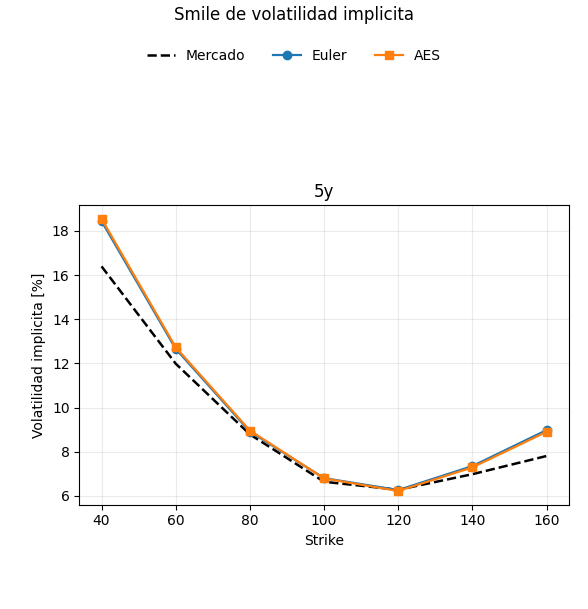
\includegraphics[width=0.5\textwidth]{AES_vs_Euler_5y.png}
    \caption{Comparación del smile de volatilidad implícita obtenido con los esquemas Euler y AES frente al smile de mercado para un vencimiento $T = 5$.}
    \label{fig:aes_euler_smile}
\end{figure}

Como se observa en la Figura \ref{fig:aes_euler_smile}, las curvas obtenidas con Euler y AES son prácticamente coincidentes para los strikes considerados. Además, ambas reproducen de forma adecuada la estructura decreciente y posterior recuperación del smile de mercado. Las pequeñas diferencias entre los dos esquemas son reducidas en comparación con el nivel de volatilidad implícita y pueden atribuirse al error de discretización y al error Monte Carlo de la simulación.\medskip

Por tanto, en este caso la elección entre Euler y AES no modifica de forma significativa los resultados finales en términos de volatilidad implícita. A continuación, se muestran y se estudian los resultados obtenidos por el esquema de Euler. \medskip

Además, tras cada paso temporal reescalamos las trayectorias de \(S(t)\) para que su media coincida con el valor
\[
    \mathbb{E}^{\mathbb{Q}}[S(t)] = S_0 e^{rt}.
\]

\subsection{Resultados obtenidos}

Los resultados principales de esta implementación son los parámetros calibrados de la componente Heston, la matriz de varianzas locales obtenida mediante Dupire y los precios de las opciones valoradas bajo el modelo Heston--SLV.

Para cada opción considerada se calcula el error absoluto entre el precio de referencia y el precio obtenido mediante SLV, siguiendo la definición dada en \ref{eq:error_absoluto}. Asimismo, para resumir el ajuste global del modelo se calcula el error absoluto medio, conforme a \ref{eq:mae}.

Las tablas completas con los precios de mercado, los precios obtenidos mediante Heston--SLV y los errores correspondientes se incluyen en las Tablas \ref{tab:slv_ref_put} y \ref{tab:slv_vs_bs_call}. 
%%%%%%%%%%%%%%%%%%%%%%%%%%%%%%%%%%%%%%%%%%%%%%%%%%%%%%
\section{Implementación del método MRE}
\label{sec:implementacion_mre}

Una vez presentada anteriormente la formulación del método de Entropía Relativa Mínima y su implementación mediante Weighted Monte Carlo en esta sección describimos cómo se ha llevado a cabo su implementación numérica. \medskip

La idea central de la implementación es mantener fijas las trayectorias simuladas del subyacente y modificar únicamente las probabilidades asociadas a cada una de ellas. Por tanto, frente al modelo Heston--SLV, donde la calibración afecta directamente a la dinámica simulada, el método MRE actúa sobre la medida discreta definida por las trayectorias Monte Carlo.

\subsection{Datos de entrada y configuración inicial}

Para que la comparación con el modelo Heston--SLV sea homogénea, se utiliza el mismo valor inicial del subyacente,
\[
S_0=100,
\]
y se consideran tipo de interés libre de riesgo y tasa de dividendos nulos,
\[
r=0, \qquad q=0.
\]
La calibración se realiza con opciones europeas de tipo call. Los vencimientos considerados son
\[
T\in
\left\{
\frac{1}{52},
\frac{1}{12},
0.5,
1,
2,
5,
8,
10
\right\},
\]
que corresponden a \(1w\), \(1m\), \(6m\), \(1y\), \(2y\), \(5y\), \(8y\) y \(10y\). Los strikes utilizados como benchmark son
\[
K\in\{40,60,80,100,120,140\}.
\]

Los precios objetivo empleados en la calibración MRE son los precios obtenidos previamente con la simulación Heston--SLV para esos mismos strikes y vencimientos. De este modo, la medida posterior MRE se calibra frente a la misma referencia que después se utilizará en la comparación entre metodologías.

La simulación previa se realiza con un modelo lognormal bajo medida neutral al riesgo. En la implementación se utilizan \(N=20000\) trayectorias, una semilla fija igual a \(12345\) y variables antitéticas, con el objetivo de mejorar la reproducibilidad y reducir la variabilidad Monte Carlo. Además, en lugar de utilizar una volatilidad prior constante para todos los vencimientos, se construye una estructura temporal de volatilidad ATM a partir de los propios precios benchmark. Como valor auxiliar de respaldo se fija
\[
\sigma_{\mathrm{prior}}=0.50,
\]
que solo se utiliza si no puede extraerse alguna volatilidad implícita representativa.

\subsection{Construcción de la medida previa}

La medida previa se define sobre las trayectorias simuladas. Inicialmente, y antes de incorporar la información de mercado, todas las trayectorias se consideran equiprobables, de modo que
\[
p_i=\frac{1}{N}, \qquad i=1,\ldots,N.
\]
A continuación, sobre cada una de estas trayectorias evaluamos los payoffs descontados de las opciones benchmark consideradas en la calibración. De esta forma, construimos la matriz \(G\), denominada matriz de payoffs, cuya estructura se recoge en \ref{matriz_payoffs_MRE}.\medskip
%miarar bien lo de arbitraje

Antes de construir la matriz de payoffs utilizada en la calibración MRE, se incorpora un módulo de comprobación de arbitraje estático sobre el conjunto finito de precios benchmark. El objetivo de este paso es verificar que los precios de mercado empleados como restricciones son compatibles con, al menos, una medida de valoración libre de arbitraje. Esta comprobación se realiza antes de la interpolación o calibración, ya que un conjunto de precios con arbitraje puede impedir la convergencia del problema de entropía relativa o generar pesos posteriores financieramente inconsistentes.

Para ello, trabajamos con precios normalizados por vencimiento. Si $(D_j)$ es el factor de descuento y $(F_j)$ el forward asociado al vencimiento $(T_j)$, se define
\[
k=\frac{K}{F_j},
\qquad
c_j(k)=\frac{C_j(K)}{D_jF_j}.
\]

Las condiciones de arbitraje estático comprobadas son las siguientes:

\begin{itemize}
\item Ausencia de arbitraje vertical: para cada vencimiento, los precios de las calls normalizadas deben ser decrecientes respecto al strike. Si se ordenan los strikes normalizados como
\[
0=k_0<k_1<\cdots<k_n,
\qquad c_0=1,
\]
y se definen las pendientes discretas
\[
q_i=\frac{c_{i-1}-c_i}{k_i-k_{i-1}},
\qquad i=1,\ldots,n,
\]
debe cumplirse
\[
0\leq q_i\leq 1.
\]

\item Ausencia de arbitraje butterfly: para cada vencimiento, la función de precios normalizados debe ser convexa respecto al strike. En términos de las pendientes anteriores, esta condición equivale a exigir
\[
1\geq q_1\geq q_2\geq \cdots \geq q_n\geq 0.
\]

\item Ausencia de arbitraje calendario: para vencimientos consecutivos \(T_j<T_{j+1}\), y sobre una misma malla de strikes normalizados, los precios de las calls normalizadas deben ser crecientes con el vencimiento:
\[
c_{j+1}(k_i)-c_j(k_i)\geq 0.
\]
Es decir, una opción con mayor vencimiento no debe tener menor valor normalizado que otra con el mismo strike normalizado y vencimiento inferior.

\item Consistencia en mallas no regulares: Cuando los strikes disponibles no coinciden entre vencimientos, la comprobación directa anterior no puede aplicarse sin más. En ese caso, el problema se formula como un problema de factibilidad lineal, buscando masas marginales y acoplamientos martingala que reproduzcan los precios observados y mantengan media normalizada igual a uno.

\end{itemize}

En la implementación utilizada, esta comprobación se completa mediante un test de existencia de pesos de estado positivos. Para un conjunto finito de strikes construimos una matriz de instrumentos frente a estados posibles del subyacente y resolvemos el sistema lineal asociado. El conjunto de precios se considera libre de arbitraje si los pesos implícitos obtenidos son positivos. En caso contrario, los precios benchmark contienen una inconsistencia estática y deben revisarse antes de ser utilizados como restricciones en la calibración MRE.

%
\subsection{Restricciones de calibración}

 En primer lugar, incorporamos las restricciones de precios de opciones, cuyo objetivo es que los precios calculados bajo la medida posterior reproduzcan los precios benchmark Heston--SLV.

En segundo lugar, se añaden restricciones forward. En el caso considerado, como \(r=q=0\), estas restricciones imponen que
\[
\sum_{i=1}^{N} q_i S_i(T_j)=S_0
\]
para cada vencimiento \(T_j\). Su finalidad es que la medida posterior conserve la consistencia con la condición neutral al riesgo del subyacente.

Por último, se incorporan restricciones sintéticas de martingala entre vencimientos consecutivos. Estas restricciones se construyen agrupando las trayectorias en ventanas según el valor del subyacente en el instante inicial del intervalo. Su objetivo es preservar, de forma aproximada y local, la propiedad martingala del proceso ponderado. Así, la calibración no se limita a ajustar precios vanilla por vencimiento, sino que también controla la consistencia temporal de la medida posterior.

\subsubsection{Formulación exacta versus mínimos cuadrados ponderados}

En el estudio de Weighted Monte Carlo en \cite{articleAvellaneda, articleElices}, se distinguen dos formulaciones principales para la imposición de restricciones de calibración: el ajuste exacto (\textit{exact fitting}) y el enfoque de mínimos cuadrados ponderados (\textit{weighted least squares}).

En la formulación de ajuste exacto, las restricciones se imponen de manera rígida. Esto significa que la medida posterior debe reproducir exactamente los precios de los instrumentos benchmark, es decir:
\[
\sum_{i=1}^{N} q_i g_{ij} = C_j, \quad j = 1,\ldots,M,
\]
donde \(C_j\) es el precio de mercado del instrumento \(j\)-ésimo. Este enfoque maximiza la consistencia con los datos observados, pero requiere que los precios benchmark sean completamente consistentes entre sí y libres de arbitraje. Cuando existen pequeñas inconsistencias numéricas, mala condición del sistema de restricciones o ruido en los datos, el método exacto puede volverse inestable.

Por el contrario, la formulación de mínimos cuadrados ponderados relaja las restricciones exactas permitiendo que exista tolerancia controlada en la reproducción de precios. En lugar de imponer igualdades estrictas, se minimiza:
\[
D(p||q) + \frac{1}{2}\sum_{j=1}^{M}\omega_j\left(\sum_{i=1}^{N} q_i g_{ij} - C_j\right)^2,
\]
donde \(\omega_j > 0\) son parámetros de regularización que controlan el peso de la restricción \(j\)-ésima. Esta formulación permite:
\begin{itemize}
  \item Estabilidad numérica: evita problemas de mal condicionamiento del sistema de restricciones.
  \item Tolerancia ante inconsistencias: acepta pequeñas desviaciones de los precios benchmark cuando éstas conducen a una medida posterior más coherente.
  \item Control de la rigidez: mediante los parámetros \(\omega_j\) se puede ajustar el compromiso entre fidelidad a los datos y suavidad de la medida.
\end{itemize}

%% En esta sección describimos primero el ajuste exacto, cuyos precios y pesos posteriores se muestran en las tablas presentadas hasta ahora. De forma paralela, se ha calculado también la calibración mediante mínimos cuadrados ponderados para poder evaluar más adelante la estructura de smile \textit{forward-start}.

En esta sección describimos ambas formulaciones. En primer lugar, utilizamos el ajuste exacto para obtener los pesos posteriores y los precios recogidos en las tablas de resultados. Esta formulación permite reproducir de forma razonable los precios benchmark y proporciona valores próximos a los obtenidos con el modelo Heston--SLV. No obstante, en el análisis posterior del smile \textit{forward-start} observamos que el ajuste exacto puede presentar problemas de estabilidad y no recuperar adecuadamente la estructura de volatilidad implícita. Por este motivo, introducimos también la formulación de mínimos cuadrados ponderados, que permite obtener una medida posterior más estable para este tipo de instrumentos.\medskip

\subsection{Resolución numérica}

%% La calibración se resuelve mediante la formulación dual, asociada al problema de minimización de entropía relativa definido en \ref{eq:problema_minimizacion_wmc}. En esta fase se presenta la resolución del ajuste exacto; la formulación de mínimos cuadrados ponderados se emplea posteriormente para comparar la reconstrucción del smile \textit{forward-start}.

La calibración se resuelve mediante la formulación dual, asociada al problema de minimización de entropía relativa definido en \ref{eq:problema_minimizacion_wmc}. Inicialmente se emplea la formulación de ajuste exacto, cuyos resultados se utilizan en las tablas de comparación de precios. Posteriormente, para estudiar la estructura de volatilidad implícita en opciones \textit{forward-start}, se considera también una formulación regularizada mediante mínimos cuadrados ponderados, con el objetivo de mejorar la estabilidad numérica de la medida posterior.\medskip

La función objetivo dual modificada es:
\[
H(\lambda) = W(\lambda) + \frac{1}{2}\sum_{j=1}^{M}\omega_j\lambda_j^2,
\]
donde \(W(\lambda) = \ln Z(\lambda) - \sum_j \lambda_j C_j\) es la función dual estándar, y los parámetros \(\omega_j\) regularizan el problema. Esta formulación es equivalente a minimizar:
\[
D(p||q) + \chi^2_w = D(p||q) + \frac{1}{2}\sum_{j=1}^{M}\omega_j\left(E^p[g_j] - C_j\right)^2,
\]
donde el primer término penaliza la desviación de la medida posterior respecto a la previa, y el segundo término controla las desviaciones en los precios benchmark.

En la práctica se utilizaron pesos de regularización
\[
\omega_{\mathrm{opciones}}
=
\omega_{\mathrm{forward}}
=
\omega_{\mathrm{martingala}}
=
10^{-7}.
\]
Esta elección de pesos permite que el método reproduzca fielmente los instrumentos benchmark mientras mantiene control sobre la estabilidad numérica del problema. Los pequeños valores de \(\omega_j\) (de orden \(10^{-7}\)) garantizan que las restricciones se cumplen con gran precisión (típicamente, errores menores que \(10^{-5}\) en escala de precios), pero al mismo tiempo evitan la rigidez excesiva que caracteriza al ajuste exacto.\medskip

Este equilibrio es especialmente importante al calibrar múltiples vencimientos con smile de volatilidad pronunciado, donde el enfoque exacto podría conducir a medidas posteriores con propiedades martingala deficientes. Los resultados numéricos muestran que la formulación de mínimos cuadrados ponderados es capaz de reconstruir estructuras complejas como el smile \textit{forward-start} (Figura \ref{fig:smile_forward_start_T1_2_T2_10}) de manera más estable y coherente que el método exacto.\medskip

El problema dual \(H(\lambda)\) se resuelve mediante un método de Newton amortiguado. La elección inicial del parámetro de amortiguación es
\[
\alpha_0=0.01,
\]
y se permite aumentarlo progresivamente hasta
\[
\alpha_{\max}=1.
\]
En cada iteración se propone un paso de Newton para los multiplicadores de Lagrange. Si el paso reduce la función objetivo y no empeora de forma significativa el condicionamiento del sistema, se acepta. En ese caso, el valor de \(\alpha\) se multiplica por un factor \(2\), sin superar \(\alpha_{\max}\). Si el paso no es aceptable, se reduce dividiendo \(\alpha\) por un factor \(5\), con un máximo de \(10\) intentos de ajuste por iteración.\medskip

Además, para evitar problemas numéricos en la evaluación de la función de partición, las exponenciales las calculamos de forma estable restando previamente el máximo de las puntuaciones. Si el sistema lineal asociado al paso de Newton está mal condicionado, se añade una pequeña regularización diagonal; y, si aun así no puede resolverse de forma directa, se utiliza una resolución en mínimos cuadrados.\medskip

Los criterios de parada utilizados son una tolerancia del gradiente igual a \(10^{-8}\) y una tolerancia de precios igual a \(5\cdot 10^{-4}\). Por otra parte, el número máximo de iteraciones se fija en \(500\).

\subsection{Pesos posteriores y valoración}

Una vez obtenidos los multiplicadores óptimos, se calculan los pesos posteriores \(q_i\) mediante la expresión exponencial de la formulación dual. Estos pesos definen la nueva medida de probabilidad discreta sobre las trayectorias simuladas.

Para analizar el efecto de la calibración, no resulta práctico mostrar todos los pesos posteriores, ya que hay un peso por cada trayectoria simulada. En su lugar, se muestran algunos valores representativos en la Tabla \ref{tab:pesos_mre}. 

\begin{table}[H]
\centering
\begin{tabular}{c|ccc}
\hline
 & Mínimo & Media & Máximo \\
\hline
\(q_i\)
& \(2.62\cdot 10^{-25}\)
& \(5.00\cdot 10^{-5}\)
& \(1.79\cdot 10^{-3}\) \\
\hline
\end{tabular}
\caption{Valores representativos de los pesos posteriores obtenidos mediante MRE.}
\label{tab:pesos_mre}
\end{table}

A partir de este punto, la valoración de derivados se realiza sustituyendo la media Monte Carlo uniforme por una media ponderada. Si \(H_i\) representa el payoff descontado de un derivado en la trayectoria \(i\), su precio bajo la medida posterior se calcula como
\[
V^{\mathrm{MRE}}
=
\sum_{i=1}^{N} q_i H_i.
\]

De esta forma, la implementación MRE queda dividida en dos fases claramente diferenciadas. Primero se calibra una medida posterior que reproduce los precios benchmark y las restricciones de consistencia. Después, esa misma medida calibrada se reutiliza para valorar los instrumentos que se compararán con el modelo Heston--SLV.\medskip

Los precios obtenidos bajo la medida posterior MRE, junto con los precios de referencia utilizados en la calibración y los errores absolutos correspondientes, se recogen en las Tablas \ref{tab:wmc_vs_ref_call} y \ref{tab:wmc_vs_ref_put}.

%%%%%%%%%%%%%%%%%%%%%%%%%%%%%%%%%%%%%%%%%%%%%%%%%%%%%%

\section{Comparación de resultados}

Una vez descrita la implementación de ambas metodologías, comparamos los precios obtenidos bajo el modelo Heston--SLV y mediante el método de Entropía Relativa Mínima implementado con Weighted Monte Carlo.\medskip

 En primer lugar, vamos a estudiar opciones europeas vanilla con strikes que no han sido utilizados directamente en la calibración, con el objetivo de analizar la capacidad de interpolación del método MRE respecto al modelo SLV. En segundo lugar, consideramos opciones de tipo \textit{forward-start}, cuyo payoff depende de la evolución del subyacente entre dos fechas futuras. De este modo, las opciones europeas vanilla permiten evaluar la consistencia de la calibración y la interpolación entre strikes, mientras que las opciones \textit{forward-start} permiten estudiar diferencias más estructurales entre ambos enfoques.


\subsection{Comparación en opciones europeas vanilla}

En primer lugar, comparamos ambos métodos en la valoración de opciones europeas
vanilla de tipo call que no han sido utilizadas directamente como instrumentos
benchmark en la calibración. En concreto, consideramos los strikes
\[
K \in \{70,90,110\}.
\]


Por tanto, el objetivo de esta primera comparación es analizar la capacidad de
interpolación del método de Entropía Relativa Mínima, implementado mediante
Weighted Monte Carlo, respecto al modelo Heston--SLV. En este caso, el
modelo Heston--SLV se toma como referencia, y estudiamos si la medida posterior
obtenida mediante WMC reproduce de forma adecuada los precios de opciones
vanilla no incluidas explícitamente en las restricciones de calibración.

Para cada strike \(K\) y vencimiento \(T\), calculamos la diferencia absoluta
\[
e(K,T)
=
\left|
C^{\mathrm{WMC}}(K,T)
-
C^{\mathrm{SLV}}(K,T)
\right|,
\]
donde \(C^{\mathrm{WMC}}(K,T)\) representa el precio obtenido mediante el método
MRE/WMC y \(C^{\mathrm{SLV}}(K,T)\) el precio obtenido bajo el modelo Heston--SLV.\medskip

La Tabla \ref{tab:comparacion_vanilla_precios} recoge los precios obtenidos por
ambas metodologías para los strikes y vencimientos considerados, junto con el error
absoluto correspondiente.

\begin{table}[H]
\centering
\scriptsize
\begin{tabular}{|c|c|c|c|c|}
\hline
\textbf{Strike} & \textbf{Vencimiento} & \textbf{Precio WMC} & \textbf{Precio SLV} & \textbf{Diferencia abs.} \\
\hline
70  & 0.02  & 30.0000 & 30.0000 & 0.0000 \\
90  & 0.02  & 10.0000 & 10.0000 & 0.0000 \\
110 & 0.02  & 0.0000  & 0.0000  & 0.0000 \\
70  & 0.08  & 30.0000 & 30.0000 & 0.0000 \\
90  & 0.08  & 10.0000 & 10.0000 & 0.0000 \\
110 & 0.08  & 0.0000  & 0.0000  & 0.0000 \\
70  & 0.50  & 30.0000 & 30.0400 & 0.0400 \\
90  & 0.50  & 10.0100 & 10.1000 & 0.0900 \\
110 & 0.50  & 0.0700  & 0.0400  & 0.0300 \\
70  & 1.00  & 30.0000 & 30.0600 & 0.0600 \\
90  & 1.00  & 10.1200 & 10.2400 & 0.1200 \\
110 & 1.00  & 0.3600  & 0.0700  & 0.2900 \\
70  & 2.00  & 30.0000 & 30.0900 & 0.0900 \\
90  & 2.00  & 10.5300 & 10.8100 & 0.2800 \\
110 & 2.00  & 0.7000  & 0.5000  & 0.2000 \\
70  & 5.00  & 30.0500 & 30.4700 & 0.4200 \\
90  & 5.00  & 12.1600 & 12.5800 & 0.4200 \\
110 & 5.00  & 2.3000  & 2.2600  & 0.0400 \\
70  & 8.00  & 30.2800 & 30.9400 & 0.6600 \\
90  & 8.00  & 13.7200 & 14.0700 & 0.3500 \\
110 & 8.00  & 4.1000  & 4.0600  & 0.0400 \\
70  & 10.00 & 30.5500 & 31.2200 & 0.6700 \\
90  & 10.00 & 14.7000 & 14.9700 & 0.2700 \\
110 & 10.00 & 5.2500  & 5.2000  & 0.0500 \\
\hline
\end{tabular}
\caption{Comparación de precios WMC y Heston--SLV para opciones europeas vanilla no utilizadas como benchmark.}
\label{tab:comparacion_vanilla_precios}
\end{table}

Para sintetizar la información anterior, en la Tabla
\ref{tab:comparacion_vanilla_metricas} mostramos la diferencia media absoluta y la diferencia máxima agrupados por vencimiento.

\begin{table}[H]
\centering
\begin{tabular}{|c|c|c|c|}
\hline
 \textbf{Vencimiento} & \textbf{MAE} & \textbf{Diferencia máxima} \\
\hline
 0.02  & 0.0000 & 0.0000 \\
 0.08  & 0.0000 & 0.0000 \\
 0.50  & 0.0533 & 0.0900 \\
 1.00  & 0.1567 & 0.2900 \\
 2.00  & 0.1900 & 0.2800 \\
 5.00  & 0.2933 & 0.4200 \\
 8.00  & 0.3500 & 0.6600 \\
 10.00 & 0.3300 & 0.6700 \\
\hline
\end{tabular}
\caption{Diferencias por vencimiento para la comparación entre WMC y Heston--SLV en opciones europeas vanilla.}
\label{tab:comparacion_vanilla_metricas}
\end{table}

Las diferencias obtenidas son reducidas en todos los vencimientos considerados. Para
los vencimientos más cortos, los precios obtenidos por ambos métodos coinciden
prácticamente.\medskip

A medida que aumenta el vencimiento, las diferencias entre ambos métodos se
incrementan ligeramente. La diferencia absoluta más grande se obtiene para el strike \(K=70\)
y vencimiento \(T=10\), con una diferencia de \(0.67\). No
obstante, la diferencia media absoluta global en el conjunto de opciones analizadas es
aproximadamente \(0.17\), por lo que la discrepancia entre ambas metodologías se
mantiene moderada.

En conjunto, estos resultados muestran que la medida posterior obtenida mediante
WMC reproduce de forma razonable los precios Heston--SLV de opciones europeas
vanilla. \medskip

Sin embargo, esta comparación solo evalúa instrumentos cuyo payoff depende del
valor del subyacente en una única fecha de vencimiento. En consecuencia, permite
analizar principalmente la consistencia de las distribuciones marginales inducidas
por ambos métodos, pero no captura completamente las diferencias asociadas a la
dinámica temporal del subyacente. Por este motivo, en la siguiente subsección se
consideran opciones de tipo \textit{forward-start}, cuyo payoff depende de la evolución
del subyacente entre dos fechas futuras.



\subsection{Comparación en opciones \textit{forward-start}}

A continuación, comparamos ambos métodos en la valoración de opciones de tipo
\textit{forward-start}, cuya definición y estructura de payoff se han introducido
previamente en la Sección \ref{sec:forward_start}. A diferencia de las opciones
europeas vanilla analizadas en la sección anterior, estos instrumentos dependen
de la evolución del subyacente entre dos fechas futuras \(T_1\) y \(T_2\), con
\(0<T_1<T_2\). Por tanto, su valoración no está determinada únicamente por la
distribución marginal del subyacente en el vencimiento final, sino también por la dinámica conjunta entre ambas fechas.\medskip

En esta comparación se consideran opciones call \textit{forward-start} para los strikes
\[
K \in \{70,90,110\},
\]
y distintos intervalos de tiempos \((T_1,T_2)\) tomados de la misma malla temporal
utilizada en la simulación. En concreto,
\[
\begin{aligned}
(T_1,T_2) \in \{&
(0.5,1),(0.5,2),(0.5,5),(0.5,10),\\
&(1,2),(1,5),(1,10),(2,5),(2,10),(5,10)\}.
\end{aligned}
\]
Esta elección nos permite analizar tanto el efecto de aumentar el vencimiento final
\(T_2\) para una fecha de inicio fija, como el efecto de retrasar la fecha de inicio
\(T_1\) para un mismo vencimiento final.\medskip

Para cada strike \(K\) y cada par de fechas \((T_1,T_2)\), se calcula la diferencia absoluta
\[
e(K,T_1,T_2)
=
\left|
C^{\mathrm{WMC}}(K,T_1,T_2)
-
C^{\mathrm{SLV}}(K,T_1,T_2)
\right|,
\]
donde \(C^{\mathrm{WMC}}\) y \(C^{\mathrm{SLV}}\) denotan, respectivamente, los
precios del contrato \((K,T_1,T_2)\) calculados con MRE/WMC y con el modelo
Heston--SLV.

La Tabla \ref{tab:comparacion_forward_start_call_precios} recoge la comparación
punto a punto de los precios obtenidos mediante ambas metodologías.

\begin{table}[H]
\centering
\scriptsize
\begin{tabular}{|c|c|c|c|c|c|}
\hline
\(T_1\) & \(T_2\) & Strike & Precio WMC & Precio SLV & Diferencia abs. \\
\hline
0.50 & 1.00  & 70  & 30.0000 & 30.0500 & 0.0500 \\
0.50 & 1.00  & 90  & 10.0200 & 10.1600 & 0.1400 \\
0.50 & 1.00  & 110 & 0.0800  & 0.1200  & 0.0400 \\
\hline
0.50 & 2.00  & 70  & 30.0000 & 30.0900 & 0.0900 \\
0.50 & 2.00  & 90  & 10.3400 & 10.7100 & 0.3700 \\
0.50 & 2.00  & 110 & 0.4200  & 0.2900  & 0.1300 \\
\hline
0.50 & 5.00  & 70  & 30.0300 & 30.4800 & 0.4500 \\
0.50 & 5.00  & 90  & 11.9400 & 12.4900 & 0.5500 \\
0.50 & 5.00  & 110 & 2.0700  & 2.0900  & 0.0200 \\
\hline
0.50 & 10.00 & 70  & 30.5000 & 31.2000 & 0.7000 \\
0.50 & 10.00 & 90  & 14.5400 & 14.9000 & 0.3600 \\
0.50 & 10.00 & 110 & 5.1300  & 5.0600  & 0.0700 \\
\hline
1.00 & 2.00  & 70  & 30.0000 & 30.0900 & 0.0900 \\
1.00 & 2.00  & 90  & 10.1200 & 10.5000 & 0.3800 \\
1.00 & 2.00  & 110 & 0.1600  & 0.1200  & 0.0400 \\
\hline
1.00 & 5.00  & 70  & 30.0200 & 30.4500 & 0.4300 \\
1.00 & 5.00  & 90  & 11.6700 & 12.3300 & 0.6600 \\
1.00 & 5.00  & 110 & 1.7500  & 1.8400  & 0.0900 \\
\hline
1.00 & 10.00 & 70  & 30.4300 & 31.1600 & 0.7300 \\
1.00 & 10.00 & 90  & 14.3600 & 14.7700 & 0.4100 \\
1.00 & 10.00 & 110 & 4.8900  & 4.9000  & 0.0100 \\
\hline
2.00 & 5.00  & 70  & 30.0000 & 30.2700 & 0.2700 \\
2.00 & 5.00  & 90  & 11.2600 & 11.8200 & 0.5600 \\
2.00 & 5.00  & 110 & 1.4800  & 1.2900  & 0.1900 \\
\hline
2.00 & 10.00 & 70  & 30.3600 & 30.9500 & 0.5900 \\
2.00 & 10.00 & 90  & 14.0400 & 14.3900 & 0.3500 \\
2.00 & 10.00 & 110 & 4.6600  & 4.5200  & 0.1400 \\
\hline
5.00 & 10.00 & 70  & 30.1100 & 30.4600 & 0.3500 \\
5.00 & 10.00 & 90  & 12.7400 & 13.1300 & 0.3900 \\
5.00 & 10.00 & 110 & 3.2100  & 3.0300  & 0.1800 \\
\hline
\end{tabular}
\caption{Comparación de precios WMC y Heston--SLV para opciones call \textit{forward-start}.}
\label{tab:comparacion_forward_start_call_precios}
\end{table}

Para resumir los resultados anteriores, en la Tabla
\ref{tab:comparacion_forward_start_call_metricas} mostramos la diferencia media
absoluta y la diferencia máxima agrupadas por cada par de fechas \((T_1,T_2)\).

\begin{table}[H]
\centering
\begin{tabular}{|c|c|c|c|}
\hline
\(T_1\) & \(T_2\) & MAE & Diferencia máxima \\
\hline
0.50 & 1.00  & 0.0767 & 0.1400 \\
0.50 & 2.00  & 0.1967 & 0.3700 \\
0.50 & 5.00  & 0.3400 & 0.5500 \\
0.50 & 10.00 & 0.3767 & 0.7000 \\
1.00 & 2.00  & 0.1700 & 0.3800 \\
1.00 & 5.00  & 0.3933 & 0.6600 \\
1.00 & 10.00 & 0.3833 & 0.7300 \\
2.00 & 5.00  & 0.3400 & 0.5600 \\
2.00 & 10.00 & 0.3600 & 0.5900 \\
5.00 & 10.00 & 0.3067 & 0.3900 \\
\hline
\end{tabular}
\caption{Métricas de error por intervalos de tiempos para opciones call \textit{forward-start}.}
\label{tab:comparacion_forward_start_call_metricas}
\end{table}

Los resultados muestran que las diferencias entre WMC y Heston--SLV son, en
general, moderadas, aunque superiores a las observadas en la comparación de
opciones europeas vanilla. Este comportamiento es esperable, ya que las opciones
\textit{forward-start} dependen de la evolución del subyacente entre dos fechas futuras y,
por tanto, son más sensibles a la dinámica temporal inducida por cada metodología.\medskip

Observamos que, para una fecha de inicio $T_1$ fija, las diferencias tienden a aumentar
cuando se incrementa el vencimiento final $T_2$. Por ejemplo, para $T_1=0.5$,
el MAE pasa de $0.0767$ en el par $(0.5,1)$ a $0.3767$ en el par
$(0.5,10)$. De forma similar, para $T_1=1$, el MAE aumenta desde $0.1700$
en $(1,2)$ hasta $0.3833$ en $(1,10)$. Esto indica que las diferencias entre
las metodologías se hacen más visibles en horizontes temporales más largos.\medskip

La mayor diferencia absoluta se obtiene para el par \((T_1,T_2)=(1,10)\) y strike
$K=70$, con una diferencia de $0.73$. También se observan diferencias relevantes
para el strike $K = 90$, especialmente en los pares $(1,5) \text{ y } (2,5)$, con diferencias
de $0.66 \text{ y } 0.56$, respectivamente. En cambio, para $K=110$ las diferencias
son más reducidas en términos absolutos.\medskip

La diferencia media absoluta global sobre las treinta opciones \textit{forward-start} consideradas
es aproximadamente $0.2943$. Este valor es mayor que el obtenido en la comparación
de opciones vanilla, lo que refleja que las opciones \textit{forward-start} constituyen una
prueba más exigente para ambas metodologías.\medskip

%%%%%%%%%%%%%%%%%%%%%%
Es importante destacar que los precios presentados en las tablas anteriores corresponden a la calibración mediante ajuste exacto. Como se observa, los valores obtenidos por WMC son próximos a los precios generados por Heston--SLV, por lo que en términos de precio la diferencia no es elevada. Sin embargo, esta comparación punto a punto no permite evaluar completamente la estructura de volatilidad implícita que induce cada metodología. En particular, al estudiar el smile \textit{forward-start}, la formulación exacta presenta problemas de estabilidad numérica y no se ha conseguido una calibración completa con una convergencia suficientemente robusta del método, posiblemente debido al elevado número de instrumentos de calibración considerados. Por este motivo, para el análisis de la estructura del smile se presentan los resultados obtenidos mediante la formulación regularizada de mínimos cuadrados ponderados.\medskip

\begin{figure}[H]
\centering
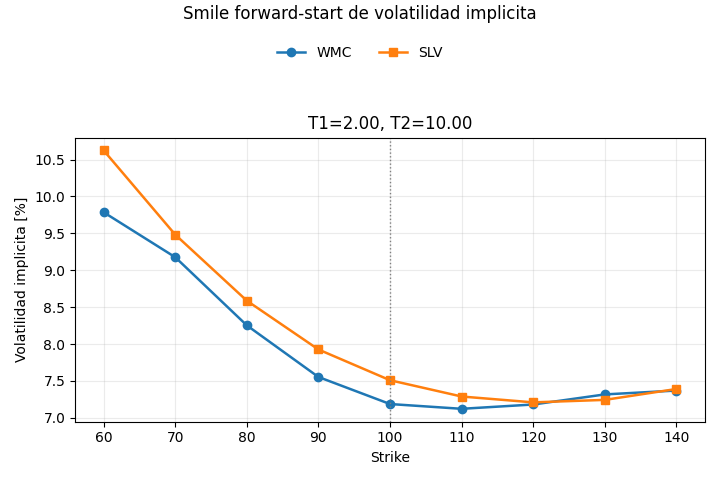
\includegraphics[width=0.75\textwidth]{wmc-slv_forward_start_WLS.png}
\caption{Smile \textit{forward-start} de volatilidad implícita para \(T_1=2\) y \(T_2=10\), obtenido con WMC calibrado por mínimos cuadrados ponderados.}
\label{fig:smile_forward_start_T1_2_T2_10}
\end{figure}

En la Figura \ref{fig:smile_forward_start_T1_2_T2_10} se muestra el smile \textit{forward-start} de volatilidad implícita para el par \((T_1,T_2)=(2,10)\), obtenido mediante WMC con calibración por mínimos cuadrados ponderados. Se observa que la curva generada por WMC reproduce de forma razonable la estructura del smile obtenida bajo Heston--SLV, capturando tanto la curvatura como el mayor nivel de volatilidad implícita para strikes bajos.\medskip

Aunque el ajuste exacto permite obtener precios próximos a los de Heston--SLV en las opciones \textit{forward-start} consideradas, los problemas de estabilidad observados al intentar recuperar la estructura completa del smile indican que esta formulación no resulta suficientemente robusta en este contexto. En cambio, la formulación de mínimos cuadrados ponderados introduce una regularización controlada de las restricciones y permite obtener una estructura de volatilidad implícita más estable.\medskip

Por tanto, los resultados ponen de manifiesto que la proximidad en precios no garantiza necesariamente una buena reproducción de la estructura de volatilidad implícita. En este sentido, el ajuste exacto resulta útil para analizar la aproximación punto a punto de precios, mientras que la formulación de mínimos cuadrados ponderados ofrece un comportamiento más adecuado cuando se estudian instrumentos más sensibles a la dinámica temporal, como las opciones \textit{forward-start}.\medskip

Por su parte, el modelo Heston--SLV incorpora una dinámica estocástica de la volatilidad combinada con una componente local, lo que le permite generar de forma natural una estructura forward de volatilidad más rica. Por ello, las opciones \textit{forward-start} permiten poner de relieve diferencias entre las metodologías que no se aprecian con la misma claridad en la comparación de opciones vanilla.


